\section{Performance Analysis}
\frame{\frametitle{Outline}\tableofcontents[currentsection,currentsubsection]}




%\frame
%{
%  \frametitle{Performance Analysis}
%
%  \begin{enumerate}
%  \item Information Integration / Filters with Paj\'e
%    \begin{itemize}
%    \item information creating based on existing events
%    \end{itemize}
%  \item Spatial and Temporal Aggregation with Paj\'e and Triva
%  \item Treemap Visualization with large-scale examples with Triva
%  \item Visualization with network topology information with Triva
%  \end{enumerate}
%}

\frame
{
   \frametitle{Performance Analysis}

   \begin{enumerate}
   \item Analysis considering network topology

      \begin{minipage}{\textwidth}
      \centering
      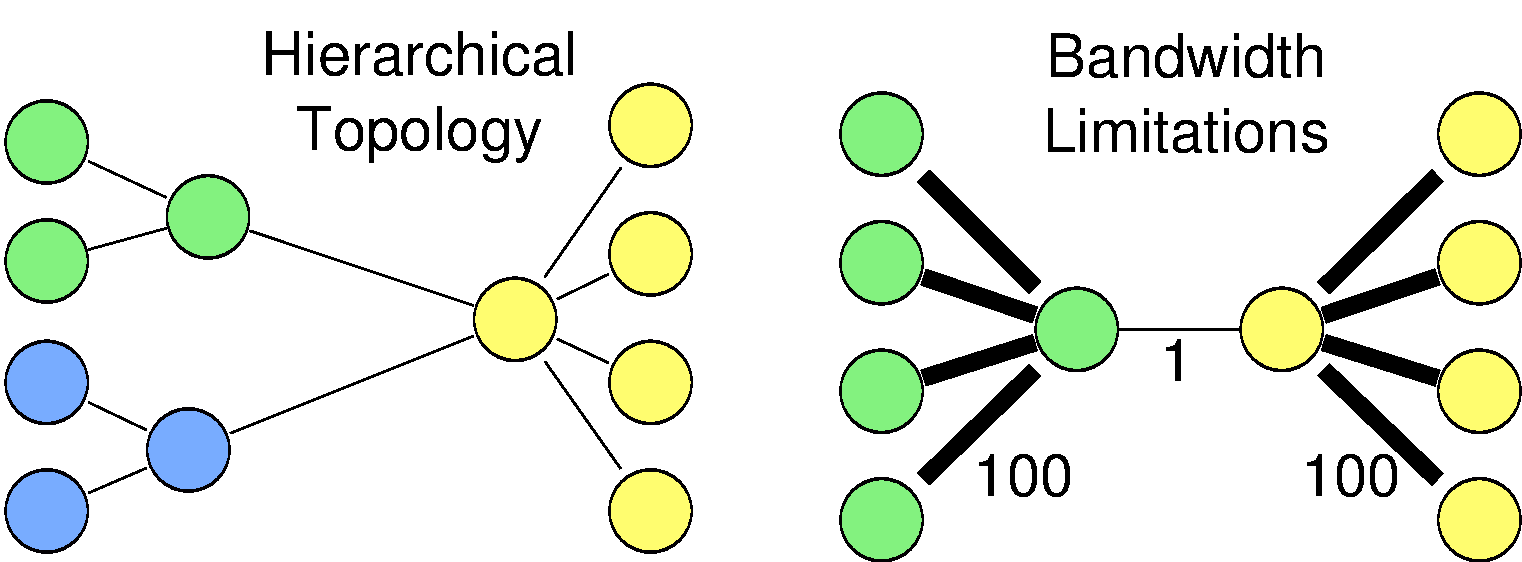
\includegraphics[width=.8\textwidth]{img/analysis-net.pdf}
      \end{minipage}

\vfill

   \item Large-scale analysis
	\begin{itemize}
	\item How to analyze thousands of processes?
	\item Temporal \& Spatial Aggregation
	\item Treemap representation
	\end{itemize}
   \end{enumerate}

   \begin{itemize}
   \item Execution Platform: Grid'5000
      \begin{itemize}
      \item Distributed resources in France
      \item Highly hierarchical network organization
      \item Limited heterogeneity -- clusters
      \end{itemize}
   \end{itemize}
}

\subsection{Three-Dimensional Model}

\frame{
   \frametitle{3D Model - Visual Conception}
   \begin{columns}
      \column{.75\textwidth}
	 \begin{itemize}
	    \item Resources represented in 2D
	       \begin{itemize}
	       \item Structural (e.g. a graph)
	       \item Statistical
	       \end{itemize}
	    \item Vertical dimension is time
	       \begin{itemize}
	       \item Objects' Behavior Evolution
	       \item States and Links
	       \end{itemize}
	       \vspace{.5cm}
	    \item Interaction Techniques
	       \begin{itemize}
		  \item Notion of a Camera
		  \item Rotation
		  \item Translation
		  \item Objects Animation
		  \item Replay step-by-step
	       \end{itemize}
	    \end{itemize}
      \column{.30\textwidth}
	 \vspace{-1cm}
	 \begin{figure}[!htb]
	 \centerline{
	    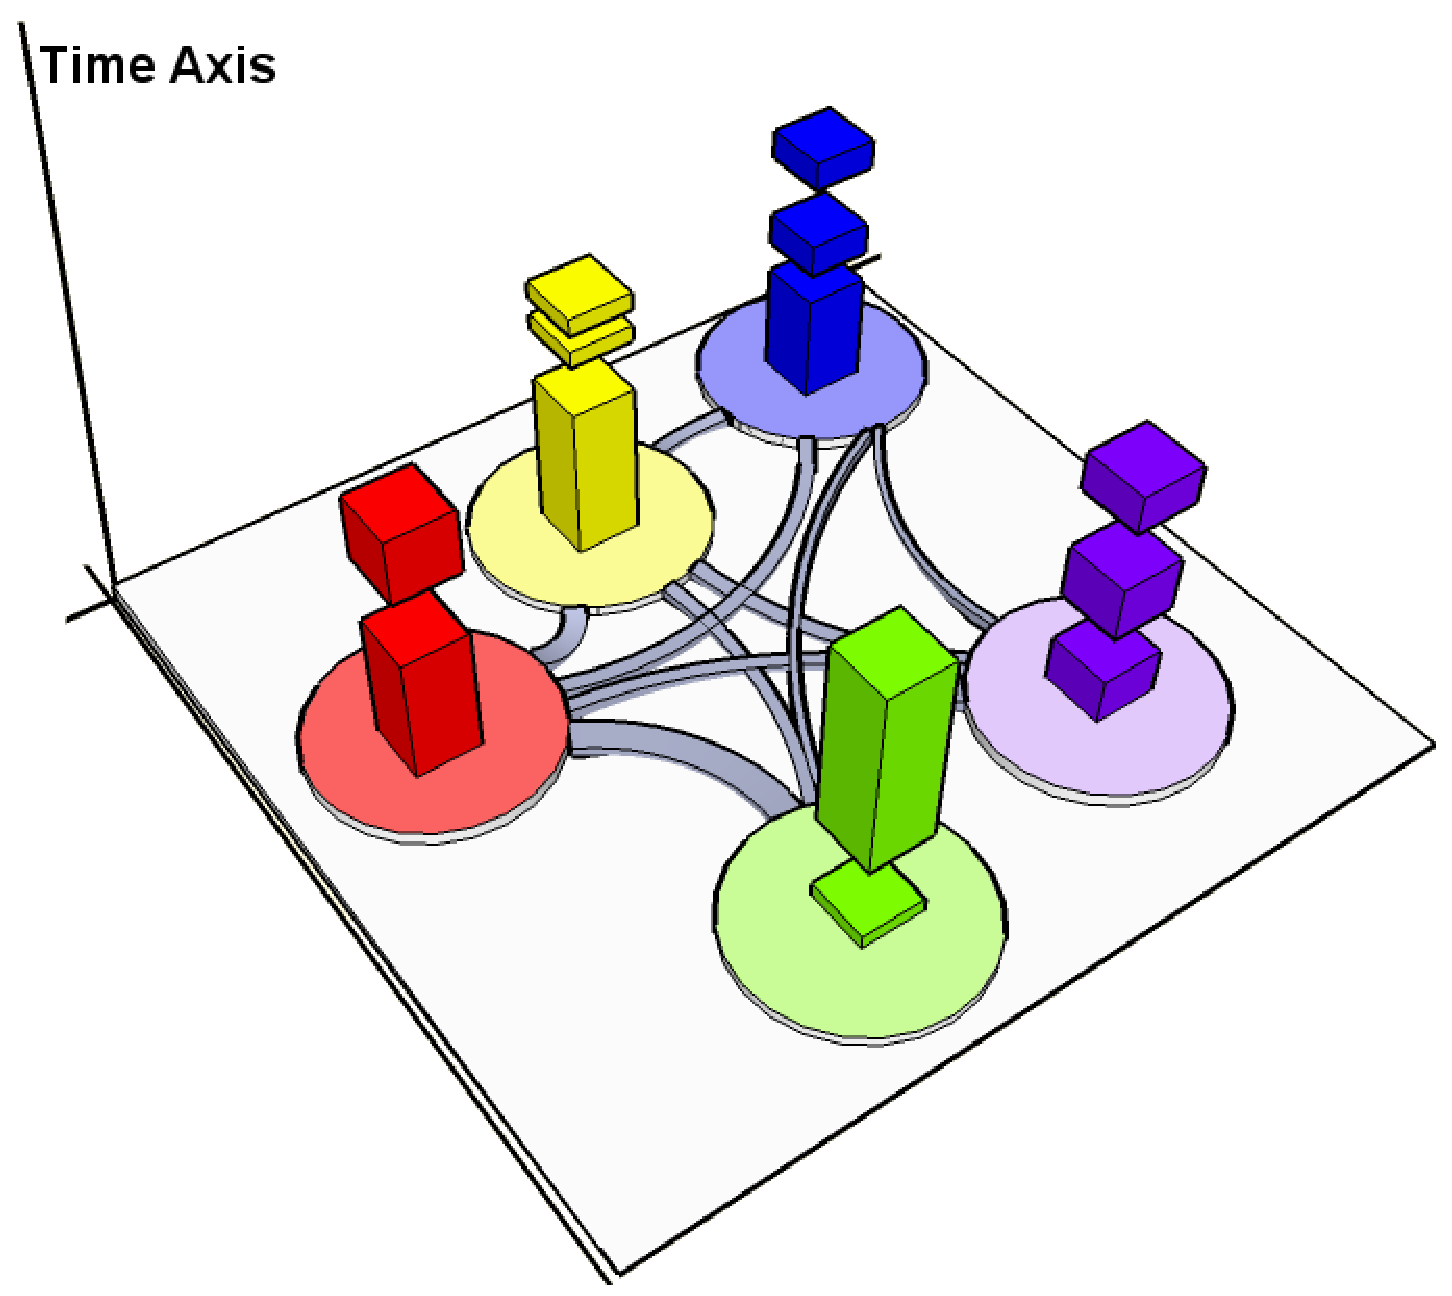
\includegraphics[width=1.2\textwidth]{img/5proc-basic-start.pdf}}
	 \centerline{
	    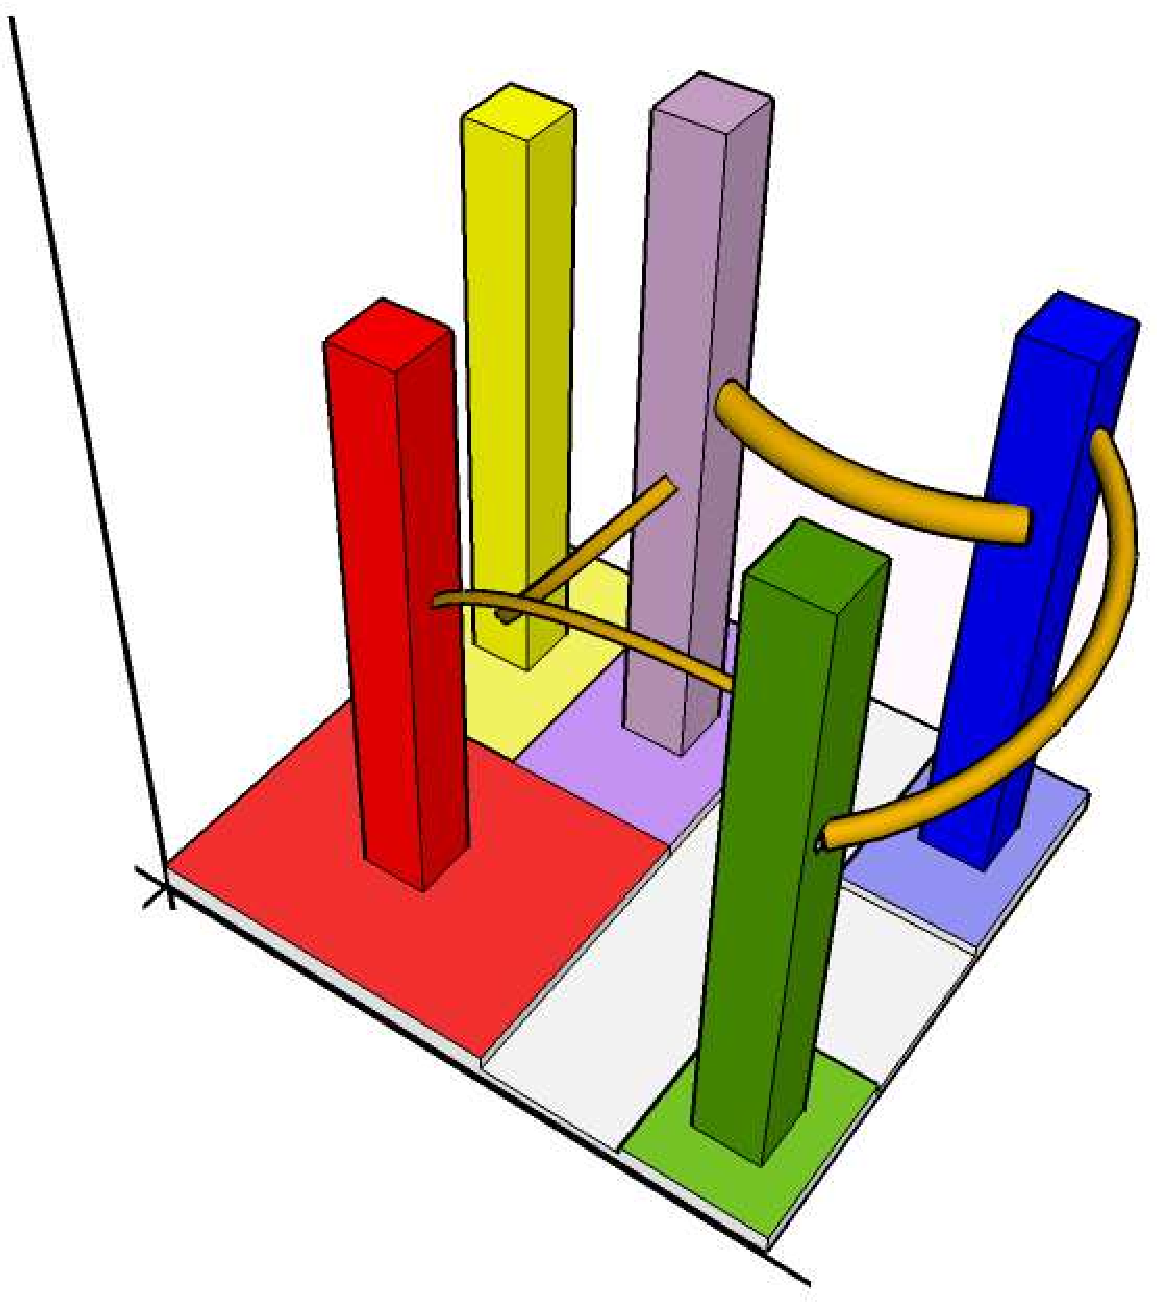
\includegraphics[width=1.2\textwidth]{img/5proc-treemap-com.pdf}}
	 \end{figure}
   \end{columns}
}

\frame{
   \frametitle{3D Model - Differences from existing tools}
   \begin{itemize}
      \item 3D Statistical Representation
	 \begin{itemize}
	 \item Pablo $\rightarrow$ 3D Scatter Plot
	 \item Paradyn $\rightarrow$ 3D Terrain
	 \item ParaProf $\rightarrow$ Triang Mesh, 3D Bar and 3D Scatter Plot
	 \end{itemize}
      \item 3D Behavioral Representation
	 \begin{itemize}
	 \item ParaProf $\rightarrow$ 2 metrics and time
	 \item Virtue $\rightarrow$ the time-tunnel view
	 \end{itemize}
      \vspace{.5cm}
      %\item Lack of structural representation
   \end{itemize}

   \vfill

   \begin{block}{Our Approach}
   \begin{itemize}
   \item Presence of a timeline to show objects' evolution
   \item Multiple Configurations in the visualization base
   \end{itemize}
   \end{block}
}

\frame{
   \frametitle{3D Model - Visualization}
   \begin{itemize}
   \item<1-> How the visual objects are represented in 3D
   \item<2-> Rendering the visualization base
      \begin{itemize}
      \item<2-> Application Communication Pattern
      \item<3-> Network Topology + App. Communication Pattern
      \item<4-> Logical Organization of Resources
      \end{itemize}
   \end{itemize}

   \vfill

   \begin{minipage}{\textwidth}
   \centering
   \includegraphics<1>[width=\textwidth]{img/3d-states-link.pdf}
   \includegraphics<2>[width=\textwidth]{img/3d-base-case1.pdf}
   \includegraphics<3>[width=\textwidth]{img/3d-base-case2.pdf}
   \includegraphics<4>[width=\textwidth]{img/3d-base-case3.pdf}
   \end{minipage}
}

%\subsection{3D Visualization}

%\frame
%{
%   \frametitle{3D Visualization - Description}
%
%   \includegraphics[width=\textwidth]{img/simple-appgraph.pdf} 
%   \vfill
%   \includegraphics[width=\textwidth]{img/simple-resgraph.pdf}
%}


\frame
{
   \frametitle{3D Visualization - Communication Patterns}

   \begin{itemize}
   \item Differences from the space-time diagram
   \end{itemize}

   \vfill
   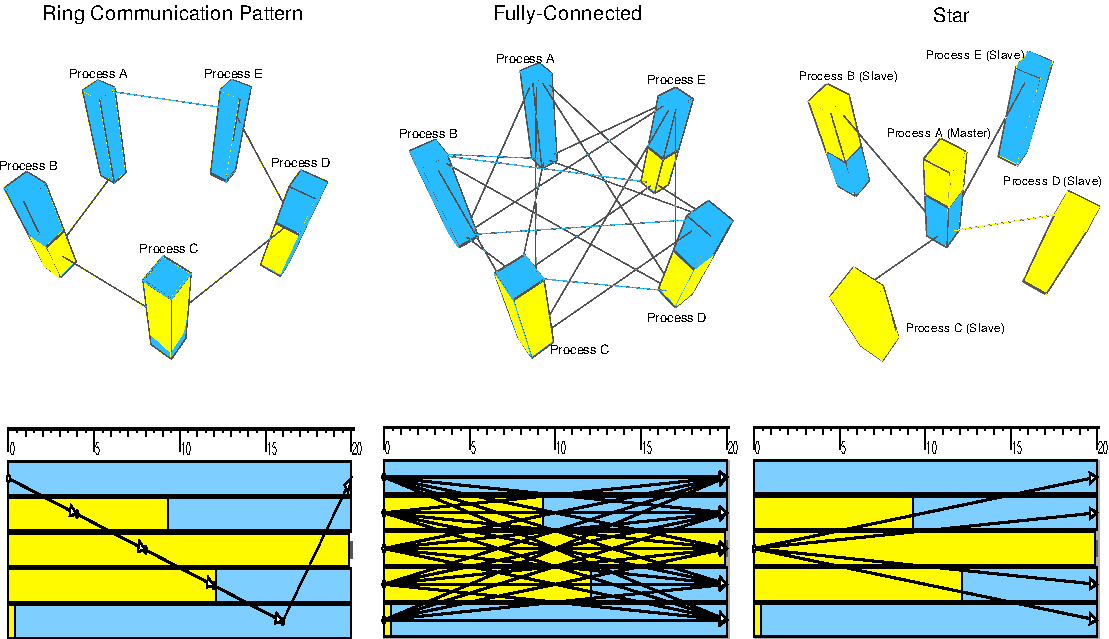
\includegraphics[width=\textwidth]{img/apppattern-ring-full-star.pdf}
   \vfill
}


\frame
{
   \frametitle{3D Visualization - KAAPI Trace}
   \begin{itemize}
   \item Fibonacci Application
   \item 26 processes, two sites, two clusters
   \item Lines represent steal requests
   \item Different number of communication between clusters
      \begin{itemize}
      \item beggining $\rightarrow$ big tasks, less communication
      \item end $\rightarrow$ smaller tasks, more communication
      \end{itemize}
   \end{itemize}

   \vfill
   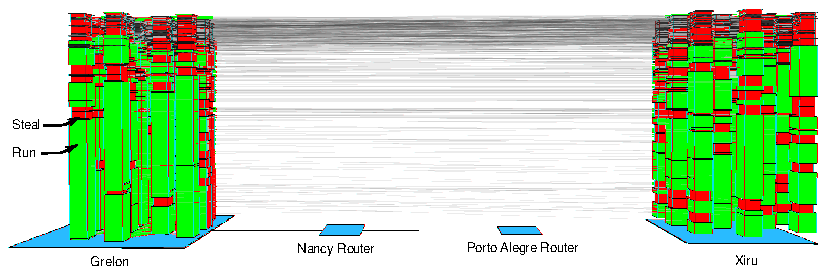
\includegraphics[width=\textwidth]{img/scenario-3d-A2.pdf}
}

\frame
{
   \frametitle{3D Visualization - KAAPI Trace}
   \begin{itemize}
   \item 60 processes, two sites, three clusters
%   \item Dashed line depicts the site separation
   \item Total execution time of a KAAPI fibonacci application
   \item Observe number of requests in time
%   \item Right image shows a larger time scale
%   \item All steal requests must go through two routers
%   \item Different stealing behavior in different intervals of time
%   \item Beggining $\rightarrow$ less requests, End $\rightarrow$ More requests
%   \item Expected behavior
   \end{itemize}

   \vfill
   \hspace{-1cm}
   \begin{minipage}{\textwidth}
   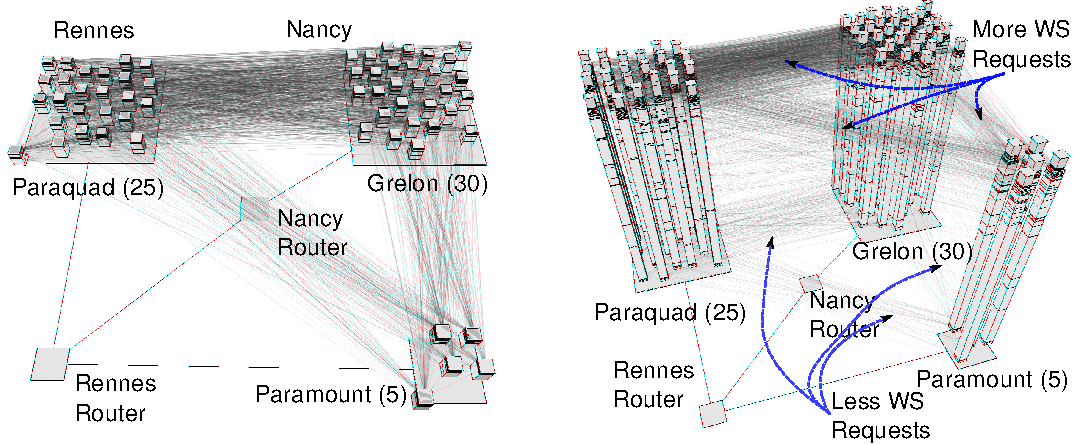
\includegraphics[width=1.15\textwidth]{img/scenario-3d-A.pdf}
   \end{minipage}
}


%\frame
%{
%   \frametitle{3D Visualization - Scenario C}
%   \begin{itemize}
%   \item 100 processes, three sites, four clusters
%   \item Visualization may suggest that big cluster allocations for this
%   particular execution should be placed in the same site
%   \item Avoiding two hops for stealing requests
%   \item Small allocations could then be placed on other sites
%   \end{itemize}
%
%   \vfill
%   \includegraphics[width=\textwidth]{img/scenario-3d-B.pdf}
%}


\frame
{
   \frametitle{3D Visualization - KAAPI Trace}
   \begin{itemize}
   \item 200 processes, 200 machines, two sites, five clusters
   \item Annotated manually with bandwidth limitations
   \end{itemize}

   \vfill
   \hspace{-1cm}
   \begin{minipage}{\textwidth}
   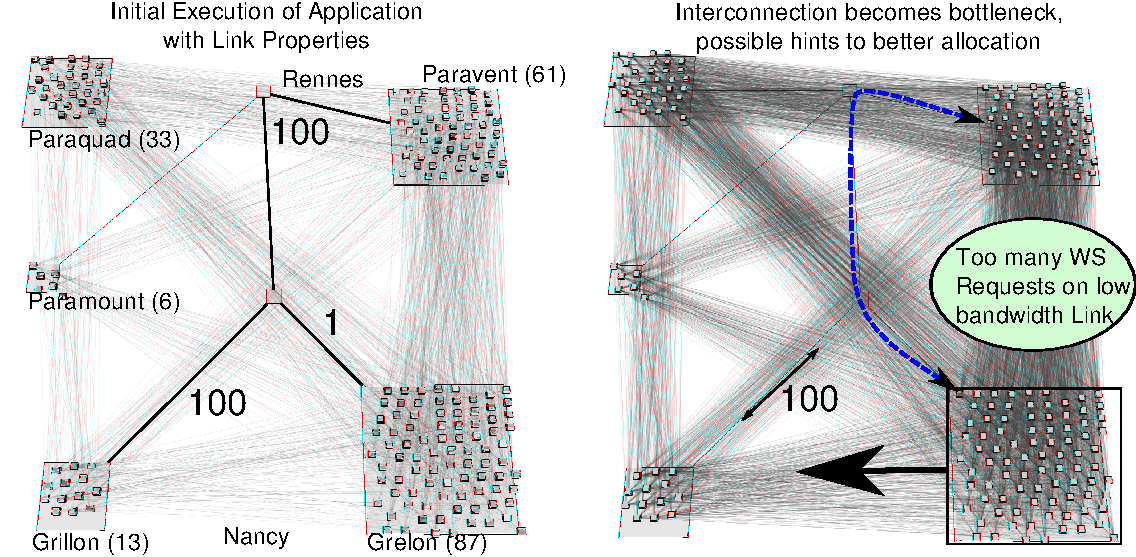
\includegraphics[width=1.15\textwidth]{img/scenario-3d-C.pdf}
   \end{minipage}
}


%\frame
%{
%   \frametitle{3D Visualization - Scenario E}
%%   \begin{itemize}
%%   \item 648 processes, two sites, five clusters
%%   \item Resulting communication pattern of KAAPI random steal requests
%%   \item Square size in the base is directly related to the number of
%%   processes in the cluster
%%   \end{itemize}
%
%   \vfill
%   \begin{center}
%   \includegraphics[width=.7\textwidth]{img/scenario-3d-D.pdf}
%   \end{center}
%}
%

\frame
{
   \frametitle{3D Visualization - KAAPI Trace}
   \begin{itemize}
   \item 2900 processes, four sites, thirteen clusters
   \end{itemize}
%   \item Illustrate different work stealing patterns that arise in different intervals of time
%   \end{itemize}
% autre façon de voir l'evolution temporelle

   \vfill
   \hspace{-1cm}
   \begin{minipage}{\textwidth}
   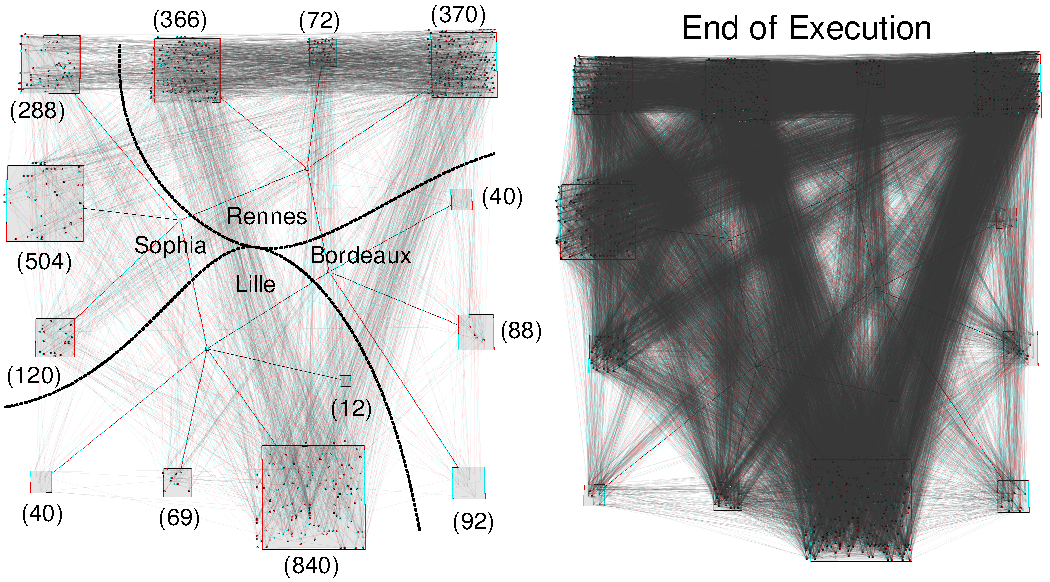
\includegraphics[width=1.15\textwidth]{img/scenario-3d-E.pdf}
   \end{minipage}
}


\subsection{Visual Aggregation Model}
\frame{\frametitle{Outline}\tableofcontents[currentsection,currentsubsection]}


\frame
{
   \frametitle{Aggregation Model - Overview}
   \begin{itemize}
   \item Enable large-scale trace analysis
   \item Visualy compare entities behavior
   \item Detect global and local characteristics

   \vfill

   \begin{block}{Steps of the Model}
      \begin{enumerate}
      \item Hierarchical Monitoring Data
      \item Compute values with the Time-Slice algorithm
      \item Apply the aggregation model
      \item Treemap representation
      \end{enumerate}
   \end{block}

   \vfill
   \item Differences from existing tools
      \begin{itemize}
      \item PlanetLab's CoVisualize $\rightarrow$ resources
      \item Treemap for Workload Visualization [Stephen 2003]
      \vspace{.2cm}
      \item Lack of configurable time intervals
      \end{itemize}
   \end{itemize}
}

\frame
{
   \frametitle{Hierarchical Monitoring Data}
   \begin{itemize}
      \item Monitoring systems register entities behavior
      \item Entities can be processes and threads
      \item They can be organized as a hierarchy
	 \begin{itemize}
	    \item Logical hierarchy
	    \item Geographical Location hierarchy
	    \item Other possibilities: libraries, components
	 \end{itemize}
      \item Grid'5000 example
   \end{itemize}

   \vfill

   \begin{minipage}{\textwidth}
   \centering
   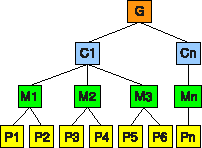
\includegraphics[width=.5\textwidth]{img/hierarchical-mon-data-4.pdf}
   \end{minipage}
}


\frame
{
   \frametitle{Time-Slice Algorithm - Basics}
   \begin{block}{Objective: annotate leaf nodes of the hierarchy}
      \begin{itemize}
      \item Time-slice definition
      \item Summary of trace events on the interval
	 \begin{itemize}
	 \item States, Variables, Links, Events, ...
	 \end{itemize}
      \end{itemize}
   \end{block}

   \vfill

   \begin{block}{Output of the Algorithm}
      \begin{itemize}
      \item Hierarchy of input
      \item Computed values on leaves
      \end{itemize}
   \end{block}

   \vfill

   \hspace{-.7cm}
   \begin{minipage}{\textwidth}
   \centering
   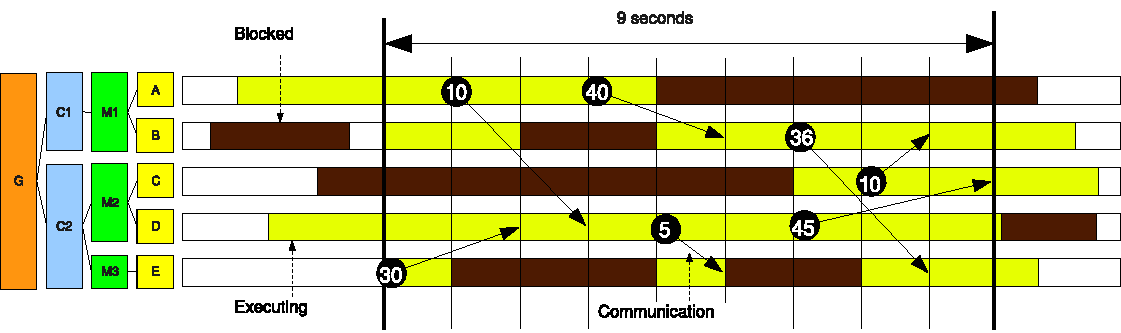
\includegraphics[width=1.1\textwidth]{img/agg-ts-complete-example.pdf}
   \end{minipage}
}

\frame
{
   \frametitle{Time-Slice Algorithm - Example}

   \hspace{-.7cm}
   \begin{minipage}{\textwidth}
   \centering
   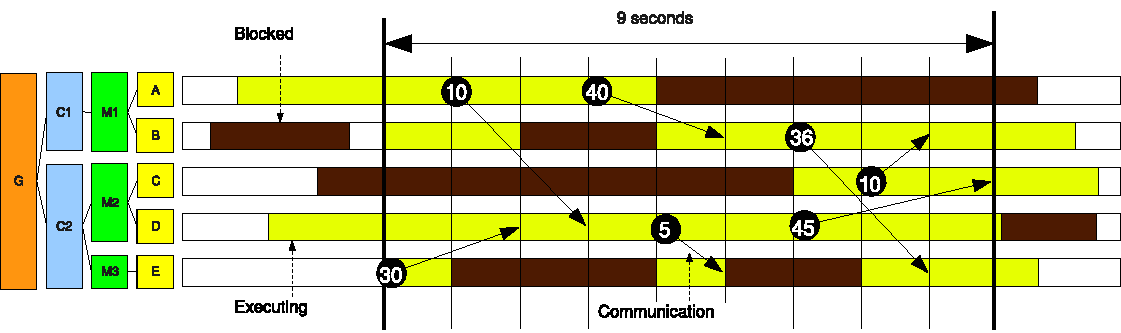
\includegraphics[width=1.1\textwidth]{img/agg-ts-complete-example.pdf}
   \end{minipage}

   \vfill

   \begin{minipage}{\textwidth}
   \centering
   \includegraphics[width=\textwidth]<1>
      {img/agg-ts-complete-example-hierarchy.pdf}
   \includegraphics[width=.75\textwidth]<2>
      {img/agg-ts-complete-example-hierarchy-merged-new.pdf}
   \end{minipage}
   
   \vfill
}



\frame
{
   \frametitle{Aggregation Model}

   \begin{itemize}
   \item Explores the hierarchical organization
   \item Creates aggregated values at intermediary levels
   \end{itemize}

   \begin{block}{Aggregation Functions}
      \begin{itemize}
      \item add, subtract, multiply, divide, ...
      \item max, min, median, average
      \item Depends on what type of value the leaves have
      \end{itemize}
   \end{block}

   \vfill

   \begin{minipage}{\textwidth}
   \centering
   \includegraphics[width=.7\textwidth]<1>{img/agg-aggmodel-overall-1.pdf}
   \includegraphics[width=.7\textwidth]<2>{img/agg-aggmodel-overall-2.pdf}
   \includegraphics[width=.7\textwidth]<3>{img/agg-aggmodel-overall-3.pdf}
   \includegraphics[width=.7\textwidth]<4>{img/agg-aggmodel-overall-4.pdf}
   \end{minipage}
}

\frame
{
   \frametitle{Visualization of the Approach - Treemaps}
   \begin{itemize}
      \item Technique created in 1991
      \item Scalable hierarchical representation
      \item Algorithm
	 \begin{itemize}
	    \item Top-down drawing
	    \item For a given node, split screen space among children
	 \end{itemize}
   \end{itemize}

   \vfill

   \begin{minipage}{\textwidth}
   \centering
   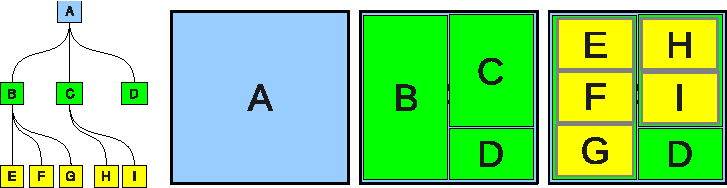
\includegraphics[width=\textwidth]{img/treemap-notion.pdf}
   \end{minipage}

   \vfill

   \begin{block}{Original algorithm has several evolutions}
   \begin{itemize}
      \item Squarified treemap is used here
      \item Keeps rectangles as close to squares as possible
   \end{itemize}
   \end{block}
}

\frame
{
   \frametitle{Treemap to view the Aggregated Hierarchy}

   \begin{minipage}{\textwidth}
   \centering
   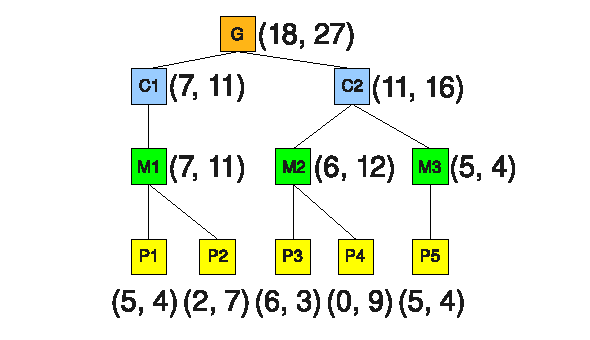
\includegraphics[width=.7\textwidth]{img/agg-aggmodel-overall-4.pdf}\\
   \includegraphics<1>[width=.28\textwidth]{img/agg-aggmodel-treemap-1.pdf}
   \includegraphics<2>[width=.28\textwidth]{img/agg-aggmodel-treemap-2.pdf}
   \includegraphics<3>[width=.28\textwidth]{img/agg-aggmodel-treemap-3.pdf}
   \includegraphics<4>[width=.28\textwidth]{img/agg-aggmodel-treemap-4.pdf}
   \end{minipage}
}

%\subsection{Treemap Visualization}

%\frame
%{
%   \frametitle{Treemap Visualization - Description}
%   \framesubtitle{Time-Slice Hierarchy}
%
%   \vfill
%   %based on img/treemap-description.svg
%   \includegraphics[width=\textwidth]{img/normal.pdf}
%}

\frame
{
   \frametitle{Treemap Visualization - Description}
   \framesubtitle{Time-Slice and Aggregated Hierarchies}

   \begin{itemize}
   \item Interaction Techniques: mouse wheel, mouse over
   \item Detailed information is available in the status bar
   \end{itemize}

   \vfill
   %based on img/treemap-description.svg
   \begin{center}
   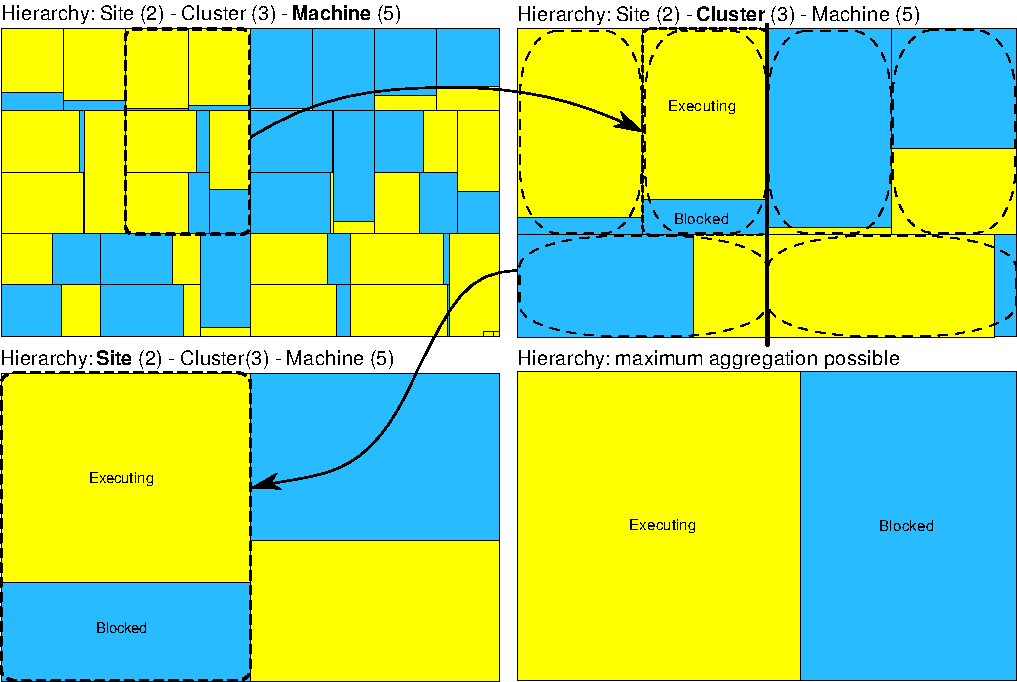
\includegraphics[width=.9\textwidth]{img/aggregated.pdf}
   \end{center}
}

\frame
{
   \frametitle{Treemap Visualization - KAAPI Trace}

%   \begin{itemize}
%   \item 2900 processes, 310 processors, four sites
%   \end{itemize}

%   \vfill
   %based on img/kaapi-scenario-c.svg
   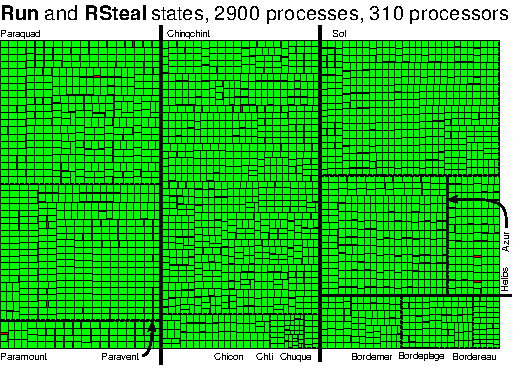
\includegraphics[width=\textwidth]{img/kaapi-scenario-c.pdf}
}


\frame
{
   \frametitle{Treemap Visualization - Large-Scale}

   \begin{itemize}
   \item Synthetic trace with 100 thousand processes
   \item Two states, four-level hierarchy
   \end{itemize}

   \vfill
   %based on img/large-scale.svg
   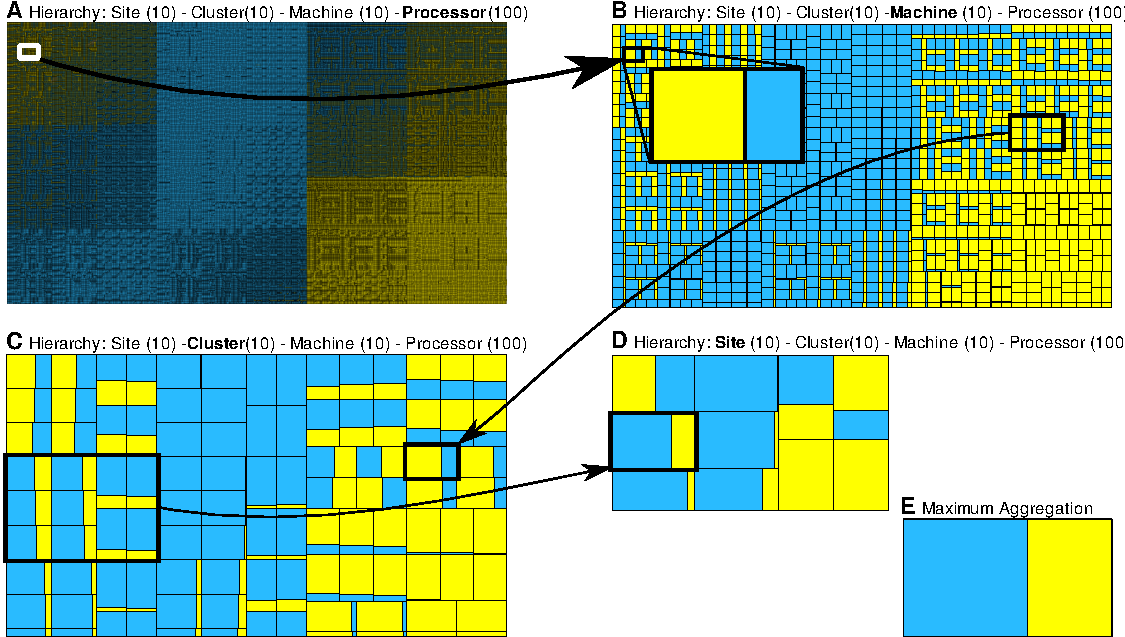
\includegraphics[width=\textwidth]{img/large-scale.pdf}
}


%\frame
%{
%   \frametitle{Treemap Visualization - KAAPI Trace}
%
%   \begin{itemize}
%   \item 200 processes, 200 machines, two sites
%   \item 100 processes per site
%   \item Different behavior: beggining/end of execution
%   \item Load-balancing between the two sites
%   \end{itemize}
%
%   \vfill
%   %based on img/kaapi-scenario-a.svg
%   \includegraphics[width=\textwidth]{img/kaapi-scenario-a.pdf}
%}


\frame
{
   \frametitle{Treemap Visualization - KAAPI Trace}

   \begin{itemize}
   \item 400 processes, 50 machines, one site
   \item 8 processes per machine
      \begin{itemize}
      \item Overload of some machines with 2 CPUs
      \item Unusual amount of time in Steal state
      \end{itemize}
   \item Machines with 4 CPUs show normal behavior
   \end{itemize}

   \vfill
   %based on img/kaapi-scenario-b.svg
   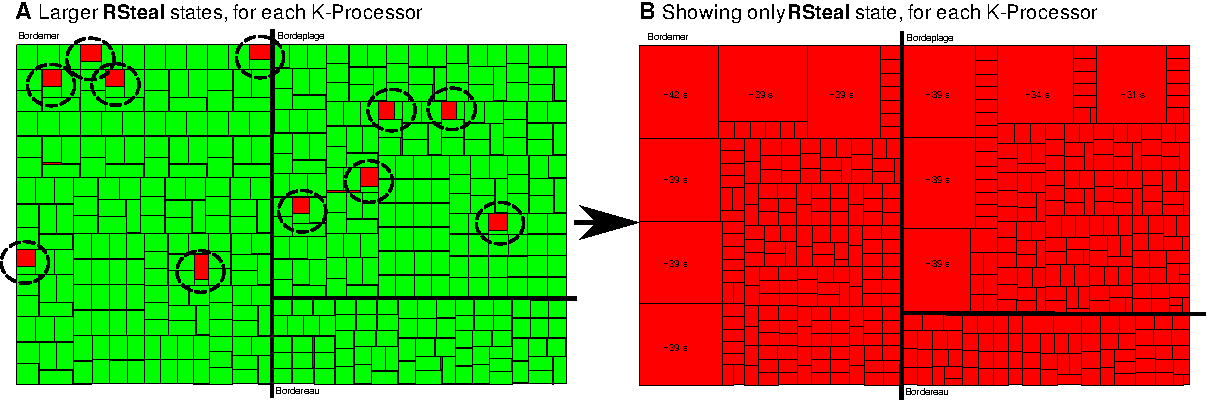
\includegraphics[width=\textwidth]{img/kaapi-scenario-b.pdf}
}

\frame
{
   \frametitle{Treemap Visualization - KAAPI Trace}

   \begin{itemize}
   \item 188 processes, 188 machines, five sites
   \item Different behavior at Porto Alegre
   \item Probably due to the interconnection
      \begin{itemize}
      \item Latency for Grid'5000 in France: \texttildelow 10 ms
      \item Latency between Porto Alegre and France: \texttildelow 300 ms
      \end{itemize}
   \item More time spent in work stealing functions
   \end{itemize}

   \vfill
   %based on img/kaapi-scenario-d.svg
   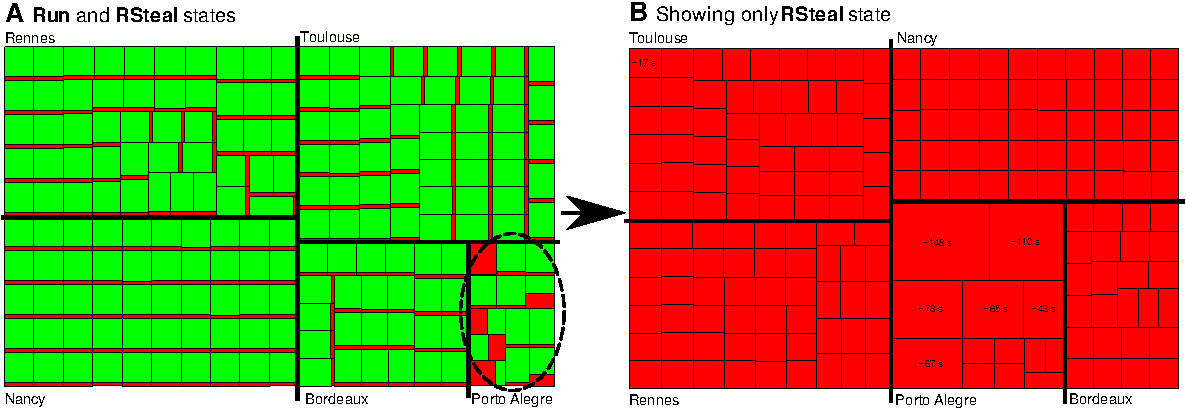
\includegraphics[width=\textwidth]{img/kaapi-scenario-d.pdf}
}

\frame
{
   \frametitle{Treemap Visualization - MPI Trace}

   \begin{itemize}
   \item Traces from the EP application -- NAS Benchmark
   \item 32 processes -- time spent in each MPI operation
   \item Init and Barrier views indicate a linear implementation
   \end{itemize}

   \vfill
   %based on img/kaapi-scenario-d.svg
   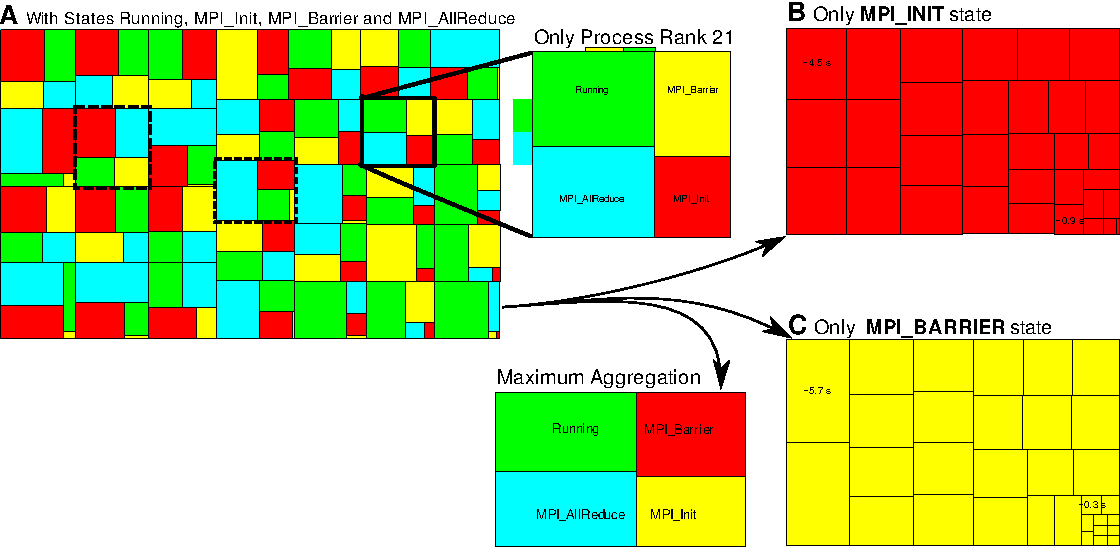
\includegraphics[width=\textwidth]{img/mpi-scenario.pdf}
}

